\section{Introduction}

RISCBoy is an open source portable games console, designed from scratch:

\begin{itemize}
\item An open source CPU, graphics and bus architecture
\item Based on the RISC-V open source instruction set
\item FPGA synthesis, place and route with icestorm open source FPGA toolchain
\item An open source PCB layout
\item PCB designed with KiCAD open source PCB software
\item It's open source
\end{itemize}

\begin{displayquote}
{\it If you say open source one more time I'm gonna nut instantly} - Oscar Wilde
\end{displayquote}

\subsection{Digital Design}

\begin{figure}[!htb]
\caption{System-level block diagram}
\label{diagram:system_arch}
\centering
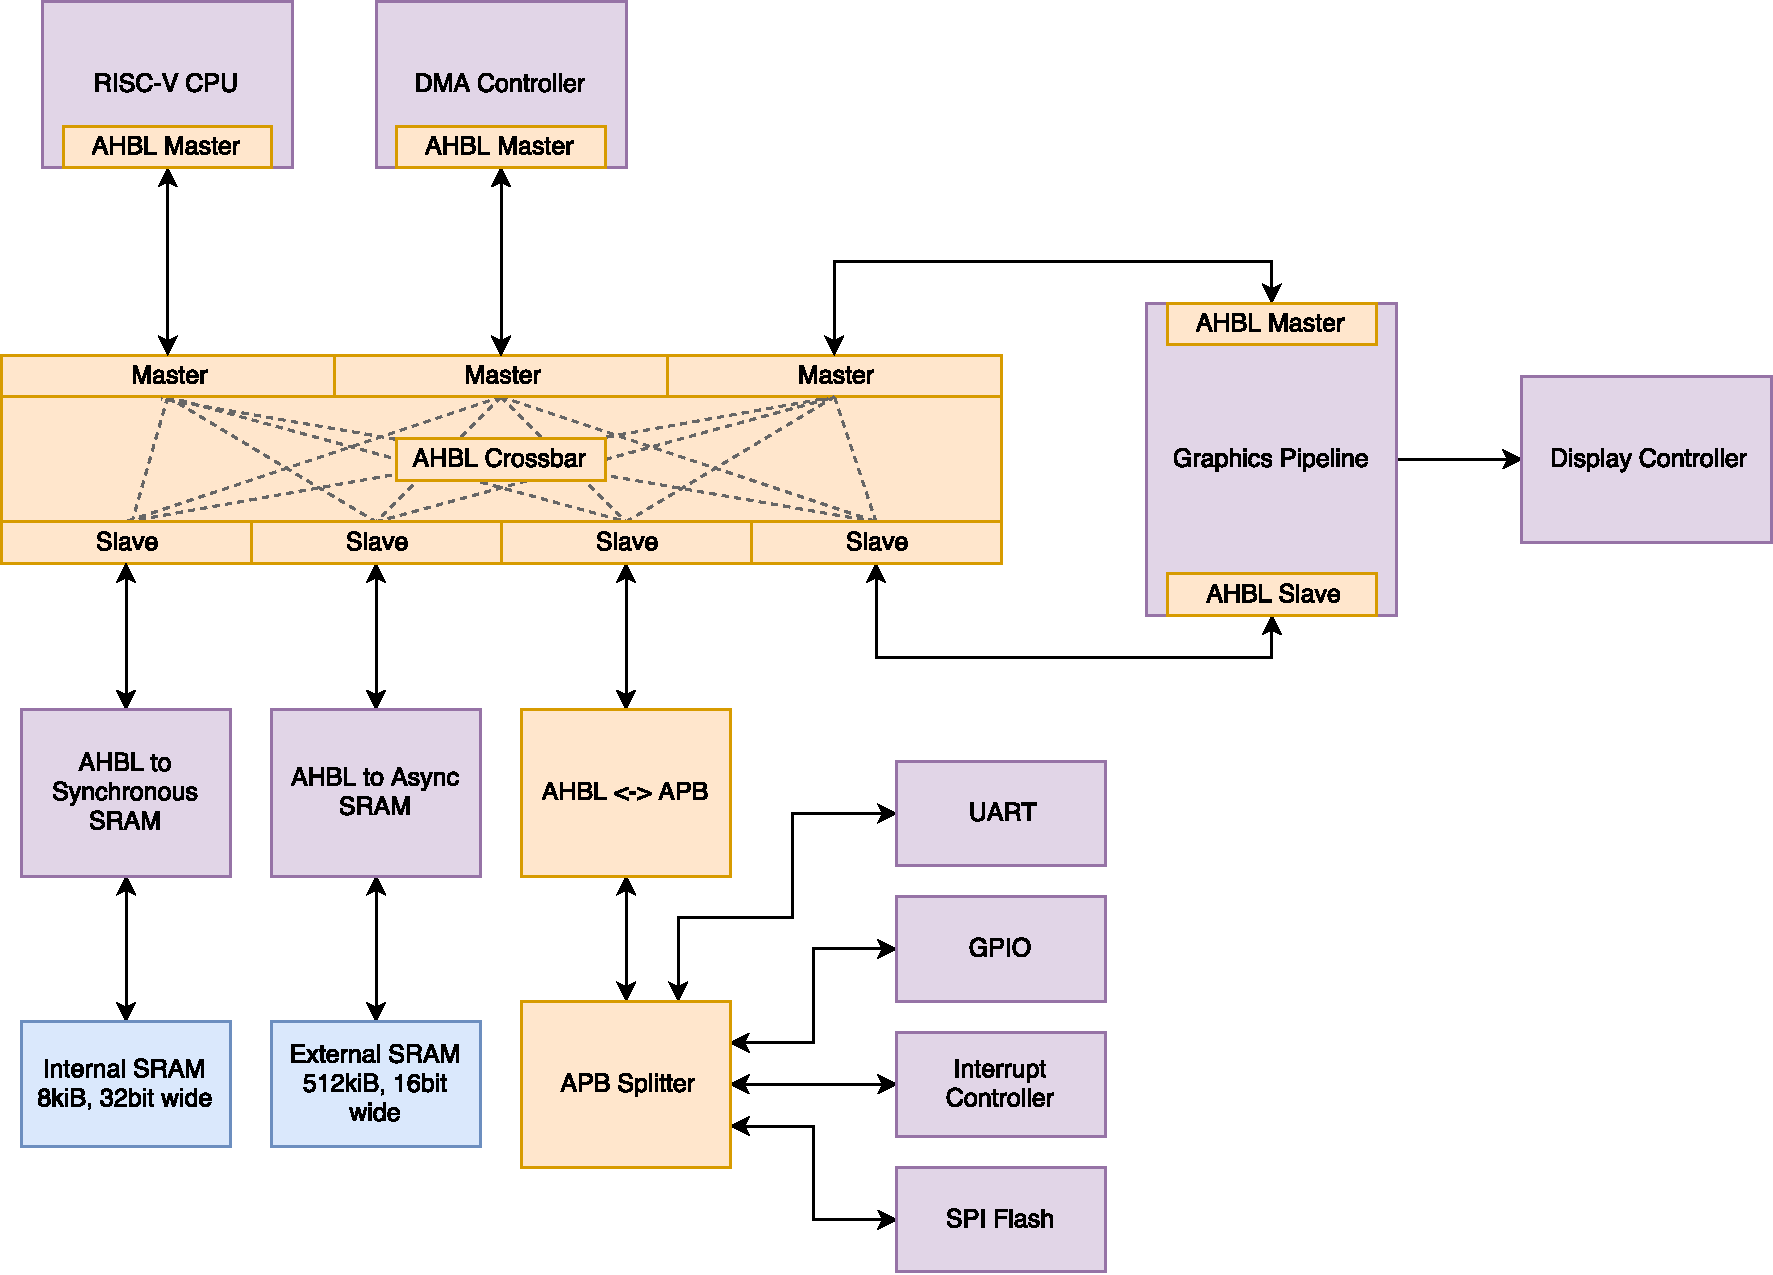
\includegraphics[width=0.7\textwidth]{diagrams/system_arch.pdf}
\end{figure}

The heart of the design is a Lattice iCE40-HX8k FPGA, containing 7680 LUT4s and flipflops. The logic was designed in synthesisable Verilog, with no dependencies on FPGA vendor IP; the contents of this GitHub repository could be taped out onto a chip. This includes:

\begin{itemize}
\item RV32IC-compatible 32-bit CPU design
	\begin{itemize}
	\item RISC-V instruction set
	\item 32I: base integer ISA profile
	\item C: compressed instruction extension, for higher code density
	\item Vectored interrupts (save/restore of PC, RA only)
	\item 5-stage pipeline, similar to textbook RISC
	\item Single AHB-Lite master port
	\end{itemize}
\item Graphics pipeline
	\begin{itemize}
	\item Don't expect much, it's about as powerful as a Gameboy Advance
	\item Includes some MODE7-like functionality which allows drawing perspective-mapped textured planes, by providing per-scanline affine texture transformation. Think MarioKart
	\end{itemize}
\item AMBA 3 AHB-Lite compatible multi-master busfabric
\item Peripherals:
	\begin{itemize}
	\item DMA master
	\item External asynchronous SRAM controller (GS74116 or similar)
	\item Display controller (ILI9341)
	\item GPIO (bitbanging, peripheral muxing)
	\item SD card controller
	\item UART
	\item PWM
	\item Basic audio: voices + samples, noise-shaped PWM output
	\end{itemize}
\end{itemize}

This document attempts to describe some of these, but if you need nitty-gritty detail, the best documentation is the files ending with {\tt .v}.

That a free synthesis tool can cram this into one of the cheapest FPGAs on the market is tremendous. I hope for a situation like software compilers, where free tools such as GCC and LLVM are industry standards.

\subsection{PCB}


\begin{figure}[!htb]
\centering
\caption{PCB stackup (left), and BGA-to-via critical clearances and dimensions (right)}
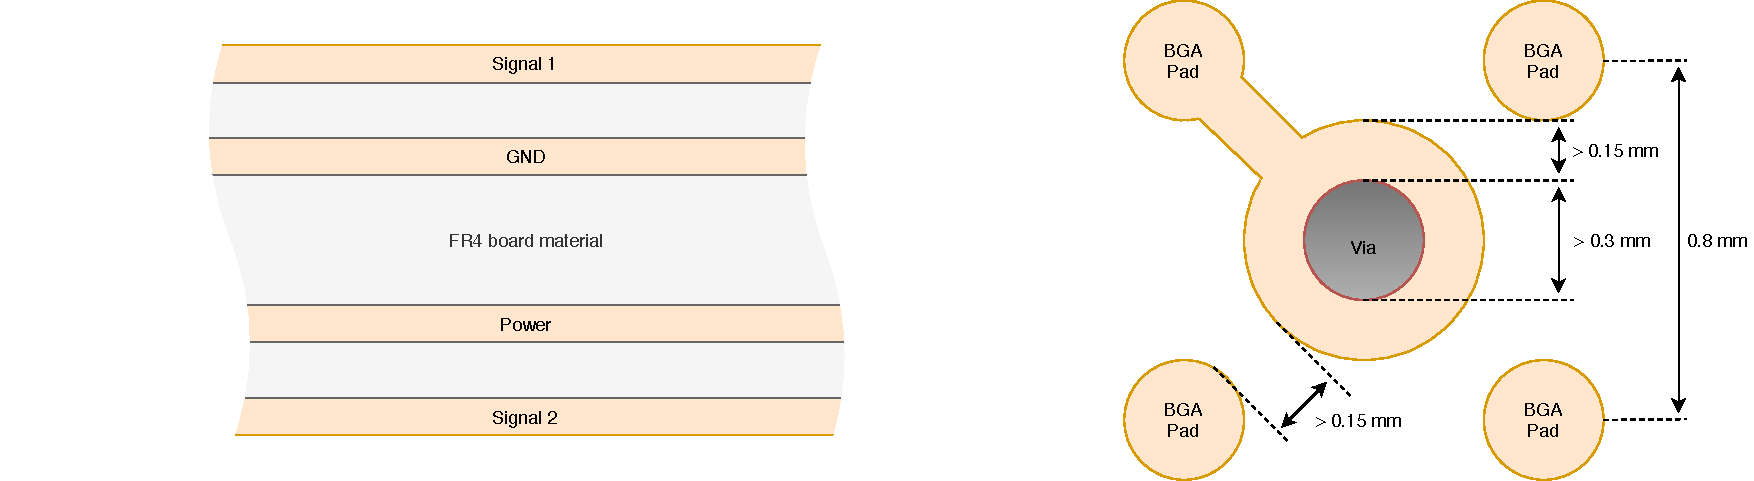
\includegraphics[width=0.8\textwidth]{diagrams/stackup_and_bga.pdf}
\label{diagram:stackup_and_bga}
\end{figure}

The board has a 4-layer stackup, illustrated in figure \ref{diagram:stackup_and_bga}. It targets low-cost PCB prototyping services such as iTead, and makes compromises to achieve this, chiefly escape routing from the FPGA ($11 \times 11$ 0.8 mm BGA). To meet iTead's copper-clearance, minimum via drill, and minimum annular ring specifications, the BGA pads must be sized down to 0.23 mm. Reflow this component by hand, with a hot air gun and plenty of flux; your toaster oven isn't going to cut it.

Schematic and layout files are in the {\tt board/} subdirectory of the git repository.

\subsection{Licensing}

The Verilog source to this project has no dependencies, and is distributed under the DWTFPL version 3. This is a {\it very} permissive open-source licence, and its text is included in full at the top of the source files. This license is very similar to the original DWTFPL, which more readers may be familiar with, but has an added indemnification clause.

This license is also known by its more formal name, as the "Do What The Fuck You Want To And Don't Blame Us Public License".